\section{asymptotically correct defect control}
\subsection{what is asymptotically correct}
Guarantees that the maximum defect is at the same place within the step.
Might want to give a paragraph on order conditions and the proof.

\subsection{derivation of asymptotically correct HB6}
To derive an asymptotically correct HB6, we thus need to use one additional function value instead of one additional y value. To that effect, we use $f_{i-2}$ instead of $y_{i+1}$ and thus we define the asymptotically correct HB6 over 3 steps and need to use a technique similar to the second HB8 scheme (See section $\ref{section:HB8_derivation}$).

In this scheme, we use 4 data points $(t_{i-1}, y_{i-1}, f_{i-1})$, $(t_{i-2}, y_{i-2}, f_{i-2})$, $(t_{i}, y_{i}, f_{i})$ and $(t_{i+1}, y_{i+1}, f_{i+1})$ with distances $\alpha h$, $h$ and then $\beta h$ between them. The middle step is the base step. This way the error term is approximately proportional to $(t- (1+\alpha))^2(t-1)^2t^2(t+\beta)^2$. We avoid the $(t-(\alpha+\beta))^2$ factor. 

The equation for the interpolant is:
\begin{equation}
\begin{split}
u(t_i + \theta h) = 
 h_id_0(\theta)f_{i-2} \\
 + d_1(\theta)y_{i-1} 
 + h_id_2(\theta)f_{i-1}\\
 + d_3(\theta)y_i 
 + h_id_4(\theta)f_i \\
 + h_id_5(\theta)f_{i+1}
\end{split}
\end{equation}
and its derivative is:
\begin{equation}
\begin{split}
u'(t_i + \theta h) = 
 d_0'(\theta)f_{i-2}\\
 + d_1'(\theta)y_{i-1}/h_i 
 + d_2'(\theta)f_{i-1}\\
 + d_3'(\theta)y_i/h_i
 + d_4'(\theta)f_i \\
 + d_5'(\theta)f_{i+1}
\end{split}
\end{equation}
Again $\theta$ is:
\begin{equation}
\theta = (t - t_i) / h_i.
\end{equation}

$\theta$ is allowed to vary between $-1-\alpha$ and $\beta$ such that $t_i + \theta h$ is $t_{i-2}$ when $\theta$ is $-1-\alpha$, $t_{i-1}$ when $\theta$ is -1, $t_i$ when $\theta$ is 0 and $t_{i + 1}$ when $\theta$ is $\beta$. Also $d_0(\theta)$, $d_1(\theta)$, $d_2(\theta)$, $d_3(\theta)$, $d_4(\theta)$ and $d_5(\theta)$ are all quintic polynomials and will each have 6 conditions from which we can build a system to find their coefficients in terms of $\alpha$ and $\beta$.

Each is a quintic of the form $a\theta^5 + b\theta^4 + c\theta^3 + d\theta^2 + e\theta^1 + f\theta$ where the six coefficients for each can be found in terms of $\alpha$ and $\beta$ by solving a linear system of 6 equations in terms of $\alpha$ and $\beta$. 

First at $\theta= -1-\alpha$, only the derivative of $d_0(\theta)$ evaluates to 1 and all other derivatives evaluate to 0. At $\theta=-1$, only $d_1(\theta)$ evaluates to 1 and other polynomials evaluate to 0 and only the derivative of $d_2(\theta)$ evaluates to 1 and all other derivatives evaluate to 0. At $\theta=0$, only $d_3(\theta)$ evaluates to 1 and other polynomials evaluate to 0 and only the derivative of $d_4(\theta)$ evaluates to 1 and all other derivatives evaluate to 0. Finally, when $\theta=\beta$, only the derivative of $d_5(\theta)$ evaluates to 1 and all other derivatives evaluate to 0. With these 6 conditions, we can get 6 equations for each quintic in terms of $\alpha$ and $\beta$ and using a symbolic management package, we can solve all of these to find the 6 coefficients for each quintic polynomial.

For the remainder of this chapter, we will denote this $6^{th}$ order asymptotic interpolant by HB6A. Its derivative has order 7 and any subsequent higher derivative will have one less order.

\subsection{using RK4 with HB6A on test problems}

\paragraph{Problem 1 results}
Figures $\ref{fig:rk4_with_hb6_asympt_p1_global_defect}$, $\ref{fig:rk4_with_hb6_asympt_p1_global_error}$ and $\ref{fig:rk4_with_hb6_asympt_p1_scaled_defects}$ shows the results of using RK4 with HB6A on Problem 1. We note that an absolute tolerance of $10^{-6}$ is applied on the maximum defect within the step and this can be shown to occur at $0.7h$ along a step of size, h. See Figure $\ref{fig:rk4_with_hb6_asympt_p1_scaled_defects}$, to see the scaled defect reaching a maximum near these points. We note that we are able to successfully control the defect of the continuous numerical solution using this approach; see Figure $\ref{fig:rk4_with_hb6_asympt_p1_global_defect}$. 

\begin{figure}[H]
\centering
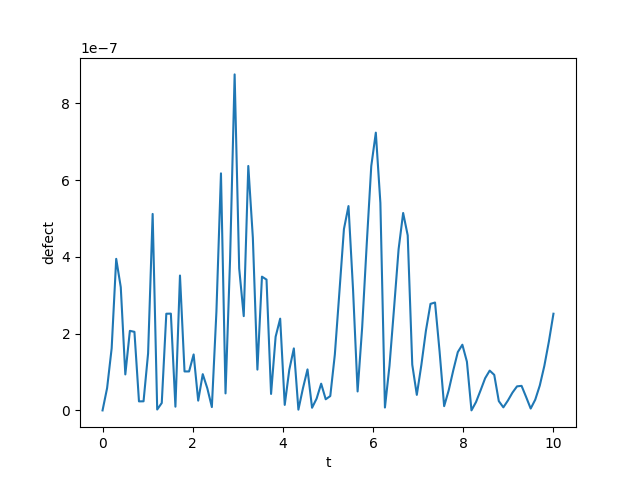
\includegraphics[width=0.7\linewidth]{./figures/rk4_with_hb6_asympt_p1_global_defect}
\caption{Defect across the entire domain for RK4 with HB6A on problem 1 at an absolute tolerance of $10^{-6}$.}
\label{fig:rk4_with_hb6_asympt_p1_global_defect}
\end{figure}

\begin{figure}[H]
\centering
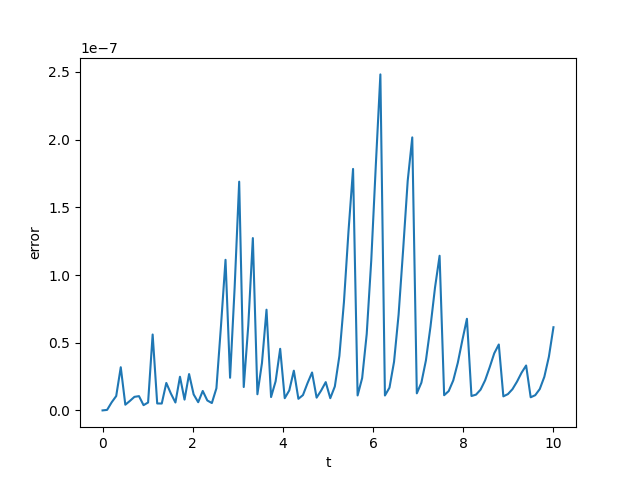
\includegraphics[width=0.7\linewidth]{./figures/rk4_with_hb6_asympt_p1_global_error}
\caption{Global Error for RK4 with HB6A on problem 1 at an absolute tolerance of $10^{-6}$.}
\label{fig:rk4_with_hb6_asympt_p1_global_error}
\end{figure}

\begin{figure}[H]
\centering
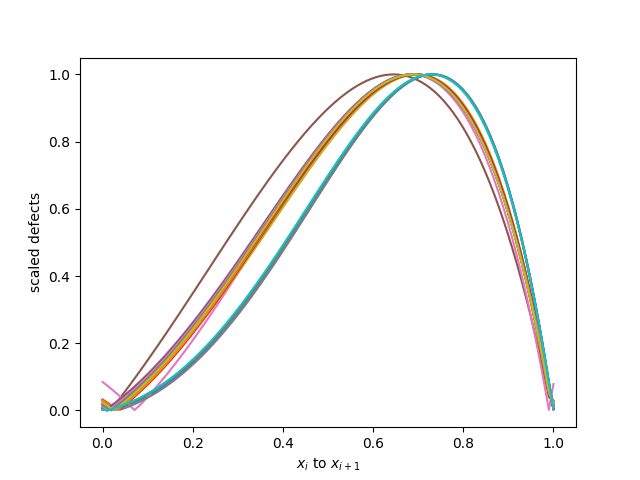
\includegraphics[width=0.7\linewidth]{./figures/rk4_with_hb6_asympt_p1_scaled_defects}
\caption{Scaled defects for RK4 with HB6A on problem 1 at an absolute tolerance of $10^{-6}$ mapped into $[0, 1]$.}
\label{fig:rk4_with_hb6_asympt_p1_scaled_defects}
\end{figure}

\paragraph{Problem 2 results}
Figures $\ref{fig:rk4_with_hb6_asympt_p2_global_defect}$, $\ref{fig:rk4_with_hb6_asympt_p2_global_error}$ and $\ref{fig:rk4_with_hb6_asympt_p2_scaled_defects}$ shows the results of using the modification of RK4 with HB6A on Problem 2. We note that an absolute tolerance of $10^{-6}$ is applied on the maximum defect within the step and this can be shown to occur at $0.7h$ along a step of size, h. See Figure $\ref{fig:rk4_with_hb6_asympt_p2_scaled_defects}$, to see the scaled defect reaching a maximum near these points. We note that we are able to successfully control the defect of the continuous numerical solution using this approach, see Figure $\ref{fig:rk4_with_hb6_asympt_p2_global_defect}$. For Problem 2, the defect is noisy on small steps and we do not get two clean peaks. However, we note that we quite consistently get the maximum defects at $0.4h$ and $0.8h$ and thus we only require two samplings.

\begin{figure}[H]
\centering
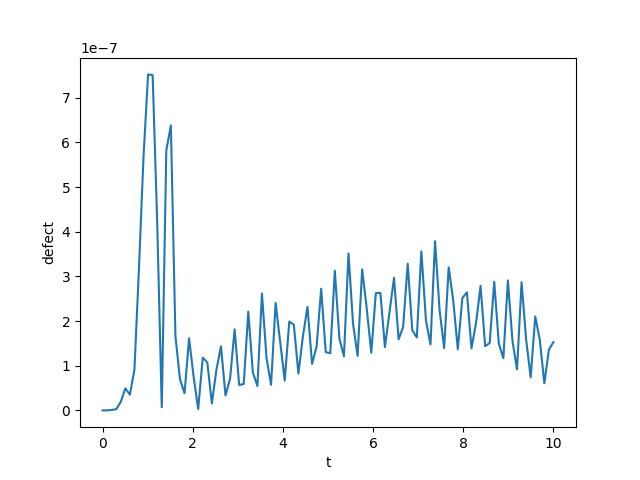
\includegraphics[width=0.7\linewidth]{./figures/rk4_with_hb6_asympt_p2_global_defect}
\caption{Defect across the entire domain for RK4 with HB6A on problem 2 at an absolute tolerance of $10^{-6}$.}
\label{fig:rk4_with_hb6_asympt_p2_global_defect}
\end{figure}

\begin{figure}[H]
\centering
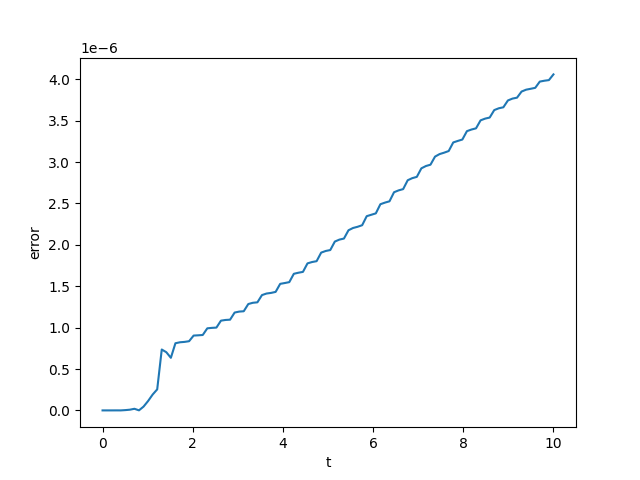
\includegraphics[width=0.7\linewidth]{./figures/rk4_with_hb6_asympt_p2_global_error}
\caption{Global Error for RK4 with HB6A on problem 2 at an absolute tolerance of $10^{-6}$.}
\label{fig:rk4_with_hb6_asympt_p2_global_error}
\end{figure}

\begin{figure}[H]
\centering
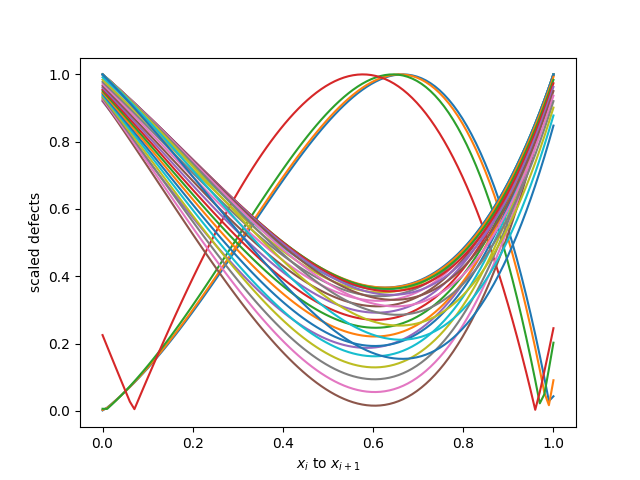
\includegraphics[width=0.7\linewidth]{./figures/rk4_with_hb6_asympt_p2_scaled_defects}
\caption{Scaled defects for RK4 with HB6A on problem 2 at an absolute tolerance of $10^{-6}$ mapped into $[0, 1]$.}
\label{fig:rk4_with_hb6_asympt_p2_scaled_defects}
\end{figure}

\begin{figure}[H]
\centering
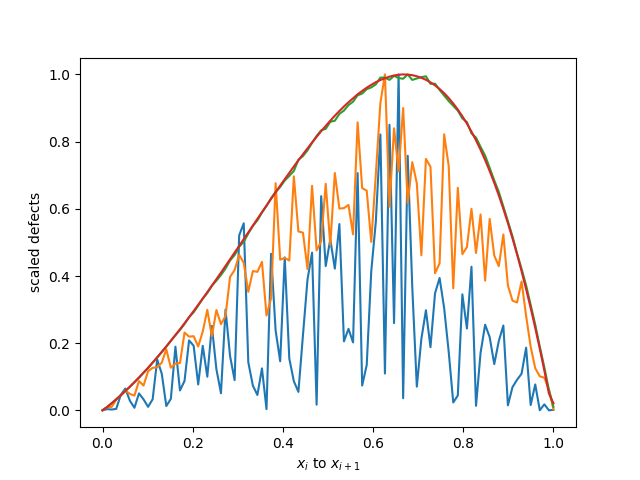
\includegraphics[width=0.7\linewidth]{./figures/rk4_with_hb6_asympt_p2_scaled_defects_small_steps}
\caption{Scaled defects for RK4 with HB6A on small steps on problem 2 at an absolute tolerance of $10^{-6}$ mapped into $[0, 1]$. Despite the noise, the maximum defect occurs near $0.8h$.}
\label{fig:rk4_with_hb6_asympt_p2_scaled_defects_small_steps}
\end{figure}

=================================================
There is a problem with the shape of the defect in this problem. For some reason, it is not 0 at the end of the steps but 1. We note that this is the exponentially increasing problem.
I think that this can be explained as we sample between $x_i$ and $x_{i+1}$ but that the interpolation point at $x_{i + 1}$ is $f_{i + 1}$ NOT $y_{i + 1}$... NEED TO CONFIRM THIS WITH THE PROF... 
==================================================


\paragraph{Problem 3 results}
Figures $\ref{fig:rk4_with_hb6_asympt_p3_global_defect}$, $\ref{fig:rk4_with_hb6_asympt_p3_global_error}$ and $\ref{fig:rk4_with_hb6_asympt_p3_scaled_defects}$ shows the results of using RK4 with HB6A on Problem 3. We note that an absolute tolerance of $10^{-6}$ is applied on the maximum defect within the step and this can be shown to occur at $0.7h$ along a step of size, h. See Figure $\ref{fig:rk4_with_hb6_asympt_p3_scaled_defects}$, to see the scaled defect reaching a maximum near these points. We note that we are able to successfully control the defect of the continuous numerical solution using this approach, see Figure $\ref{fig:rk4_with_hb6_asympt_p3_global_defect}$. 


\begin{figure}[H]
\centering
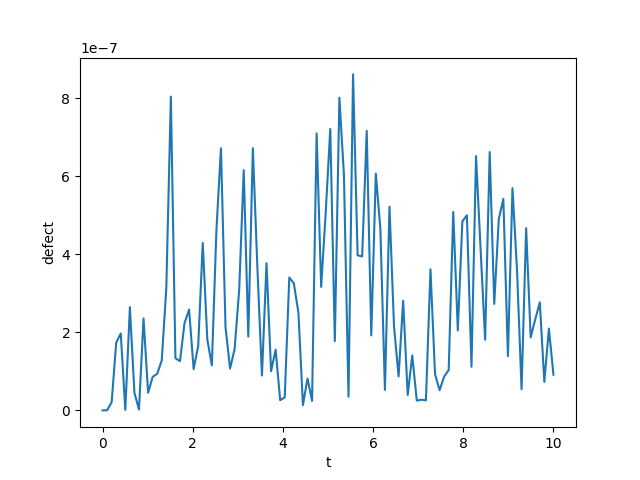
\includegraphics[width=0.7\linewidth]{./figures/rk4_with_hb6_asympt_p3_global_defect}
\caption{Defect across the entire domain for RK4 with HB6A on problem 3 at an absolute tolerance of $10^{-6}$.}
\label{fig:rk4_with_hb6_asympt_p3_global_defect}
\end{figure}

\begin{figure}[H]
\centering
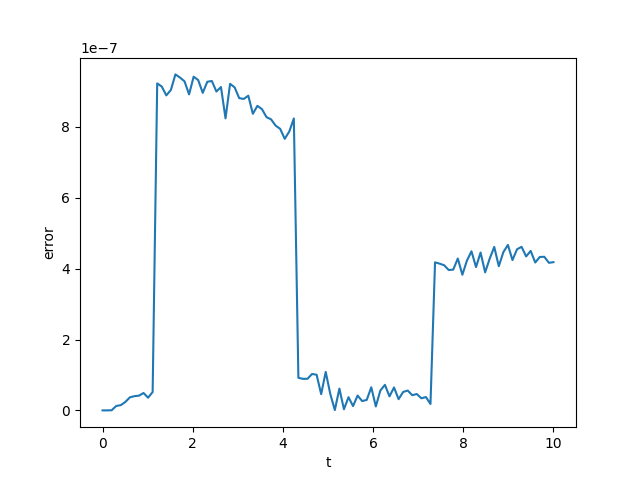
\includegraphics[width=0.7\linewidth]{./figures/rk4_with_hb6_asympt_p3_global_error}
\caption{Global Error for RK4 with HB6A on problem 3 at an absolute tolerance of $10^{-6}$.}
\label{fig:rk4_with_hb6_asympt_p3_global_error}
\end{figure}

\begin{figure}[H]
\centering
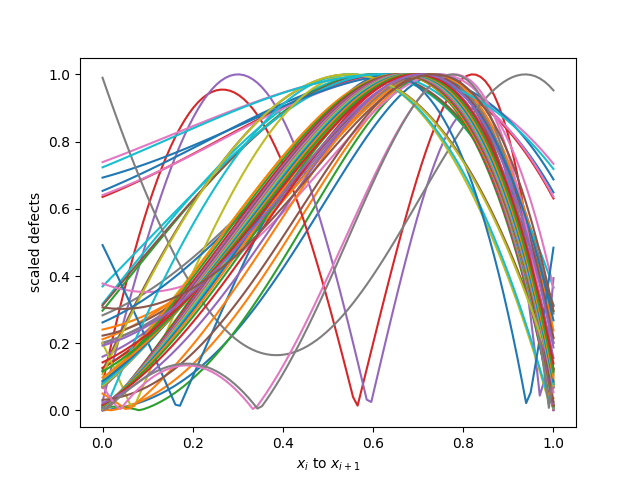
\includegraphics[width=0.7\linewidth]{./figures/rk4_with_hb6_asympt_p3_scaled_defects}
\caption{Scaled defects for RK4 with HB6AAsympt on problem 3 at an absolute tolerance of $10^{-6}$ mapped into $[0, 1]$.}
\label{fig:rk4_with_hb6_asympt_p3_scaled_defects}
\end{figure}

The shape is not a distinct peak at $0.7h$ for all steps but we were still able to control the defect.

\begin{table}[h]
\caption {Number of steps taken by RK4 when modified to do defect control with HB6 vs HB6 Asympt.} \label{tab:rk4_with_hb6_asympt_nsteps}
\begin{center}
\begin{tabular}{ c c c c c } 
Problem & succ. steps HB6A & succ. steps HB6 & nsteps HB6A  & nsteps HB6 \\ 
1       & 41               &        27       & 43           & 27 \\ 
2       & 35               &        36       & 36           & 40 \\
3       & 60               &        62       & 80           & 73 \\
\end{tabular}
\end{center}
\end{table}

From Table $\ref{tab:rk4_with_hb6_asympt_nsteps}$, we can see that RK4 with HB6A is worse than with HB6. We note that although that is the case, there is some guarantee with HB6A that we are always sampling the maximum defect but that no guarantee is made with HB6. Thus we expect, the solution provided by RK4 with HB6A to be more accurate than that of rk4 with HB6.